\chapter{Realizzazioni sperimentali e valutazione}
\label{ProveSperimentali}
\thispagestyle{empty}

\vspace{0.5cm}

\noindent Nel Capitolo \ref{SoluzioneProposta} abbiamo illustrato gli algoritmi proposti per la soluzione del tampering detection.
Tali algoritmi sono stati implementati nel linguaggio di programmazione \textit{MATLAB}, in modo valutarne le prestazioni. 
In questo capitolo illustriamo come sono stati condotti questi esperimenti.\\
Il Paragrafo \ref{acquisizione} \`e dedicato alla descrizione dei dataset utilizzati come riferimento, mostrando quali sistemi di acquisizione sono stati utilizzati e quali sono le metriche che abbiamo tenuto in considerazione.\\
Nel Paragrafo \ref{risultati}, invece, entriamo nel dettaglio su quali sono stati i risultati a valle di tutta l'analisi sperimentale. 
\section{Acquisizione dei dataset}
\label{acquisizione}
Durante lo svolgimento della tesi abbiamo acquisito diversi dataset video, in modo da poter testare le soluzioni proposte per quanto riguarda la segmentazione in regioni della scena e l'identificazione di eventi di tampering.\\
Un primo dataset \`e stato acquisito utilizzando una \textit{macchina fotografica digitale} in grado di registrare video.
Questo primo insieme \`e stato utilizzato come \textit{benchmark} per l'algoritmo di segmentazione, e comprendeva scene riprese all'aperto con un framerate elevato ($30$ fps).
Ciascun video comprendeva un minuto di ripresa ($1800$ frame), e ci\`o lo rendeva inutilizzabile per validare le scelte fatte per l'algoritmo di tampering detection.\\
Abbiamo creato, quindi, un secondo dataset utilizzando un sistema di acquisizione basato su un \textit{Raspberry Pi modello B+} \cite{raspberry} con relativo \textit{modulo camera} \cite{raspberryCamera}.
Il Raspberry Pi (Fig. \ref{fig:raspberry}) \`e un \textit{single-board computer} (ovvero un computer implementato su una singola scheda elettronica) basato su un \textit{system-on-chip} (SoC) \textit{Broadcom BCM2835} \cite{broadcom}, che incorpora un processore \textit{ARM1176JZF-S} \cite{arm}, una GPU \textit{VideoCore IV} \cite{gpu} e $512$ MB di memoria.
Utilizza un sistema operativo \textit{Debian Linux} realizzato per processori ARM chiamato \textit{Raspbian} \cite{raspbian}.\\
Il modulo camera permette di acquisire immagini a diverse risoluzioni e a diverso framerate, fornendo inoltre la possibilit\`a di salvarle in vari formati.
Abbiamo deciso, quindi, di acquisire i frame in formato non compresso \textit{yuv}, in modo da avere la maggior qualit\`a possibile.\\
Il sistema realizzato \`e illustrato nella Figura \ref{fig:raspberryC}. Le ridotte dimensioni e il basso consumo di potenza del sistema hanno permesso il suo utilizzo per fare le acquisizioni in ambienti esterni, utilizzando una batteria per alimentare il tutto. 
\begin{figure}[tb]
	\centering
	\begin{subfigure}[]
		{\includegraphics[height=6cm]{./pictures/RaspberryPiB+}
			\label{fig:raspberry}}
	\end{subfigure}
	\begin{subfigure}[]
		{\includegraphics[height=6cm]{./pictures/raspberry}
	\label{fig:raspberryC}}
	\end{subfigure}
	\caption{Il Raspberry Pi (a) e il sistema di acquisizione basato su di esso (b)}
\end{figure}
Per interfacciarci con il dispositivo abbiamo creato una \textit{connessione SSH}, tramite USB, con uno smartphone: in questo modo abbiamo potuto lanciare i comandi necessari per far partire l'acquisizione. 
Per l'acquisizione abbiamo creato uno script in \textit{Python}, utilizzando la libreria \textit{picamera} \cite{picamera} per interfacciarci con il modulo camera.\\
Abbiamo creato, infine, un terzo dataset utilizzando il sito \textit{ilMeteo.it}.
Questo portale di previsioni del tempo fornisce l'accesso ai frame acquisiti dalle webcam presenti in varie citt\`a italiane e in varie localit\`a turistiche.
A ciascuna webcam \`e associato un unico URL, in cui \`e presente un'immagine in formato \textit{jpeg} rappresentante il frame corrente acquisito dalla camera.
Queste webcam, in genere, acquisiscono un frame ogni minuto, e ci\`o ha permesso di utilizzarle come caso d'uso reale.\\
Attraverso uno script in Python e il tool \textit{curl} \cite{curl}, che permette il trasferimento di dati da indirizzi URL, abbiamo creato delle sequenze di frame che coprono un arco di $24$ ore ciascuna, con frame acquisiti ogni minuto.
In questo modo abbiamo potuto valutare il comportamento degli indicatori in condizioni di framerate basso e su lunghi periodi.
\subsection{Eventi di tampering}
Per testare i nostri algoritmi, abbiamo dovuto creare degli eventi in cui venga compromessa l'acquisizione corretta della scena ripresa.
Nel caso del dataset acquisito con il Raspberry Pi abbiamo potuto creare degli eventi di tampering \textit{reali}, ad esempio spostando la camera durante la ripresa, oppure buttando dell'acqua o spruzzando del deodorante spray sull'obiettivo della camera, in modo da creare la sfocatura.\\
Nel caso dei frame presi dalle webcam su internet abbiamo dovuto creare degli eventi di tampering in maniera \textit{artificiale}.
La sfocatura \`e stata introdotta utilizzando delle convoluzioni con filtri \textit{gaussiani} di varie dimensioni, mentre lo spostamento della camera \`e stato simulato concatenando sequenze di frame differenti.
\subsection{Definizione dei ground thruth}
Per valutare le prestazioni del nostro metodo, abbiamo dovuto definire un \textit{ground thruth} (GT) per ciascuna sequenza video, in modo da poter disporre di alcune metriche per poter confrontare i risultati ottenuti.\\
Dato che il nostro algoritmo identifica gli istanti in cui evento di tampering inizia, nel GT di ciascuna sequenza sar\`a presente, quindi, il numero del frame in cui questo evento inizia effettivamente. 
In particolare avremo un'indicazione del frame in cui avviene una sfocatura (se presente) e un'indicazione del frame in cui avviene lo spostamento della camera (se presente).
Ricordiamo, inoltre, che nella nostra analisi stiamo considerando che il passaggio da una situazione prima di tampering a una con tampering come un evento \textit{istantaneo}. 
\section{Risultati sperimentali}
\label{risultati}
L'insieme dei dataset e dei GT ci ha permesso di realizzare una piattaforma per testare le prestazioni del nostro algoritmo di tampering.
\subsection{Esperimenti condotti}
\begin{itemize}
	\item \textbf{Identificazioni di spostamenti della camera}
	\begin{itemize}
		\item energia media della luma su tutta la scena (detrending)
		\item energia media della luma sulle regioni (detrending)
		\item frame difference su tutta la scena  (detrending)
		\item frame difference sulle regioni (detrending)
	\end{itemize}
	\item \textbf{Identificazioni di sfocature}
	\begin{itemize}
		\item energia media del gradiente su tutta la scena  (detrending)
		\item energia media del gradiente sule regioni (detrending)
		\item monitoraggio sequenziale della varianza dell'energia media del gradiente
	\end{itemize}
\end{itemize}
\subsection{Definizione delle metriche per la stima delle prestazioni}
Grazie all'informazione presente nel GT siamo in grado, una volta che viene lanciato l'algoritmo di tampering detection, di definire quando il risultato \`e corretto e quando no.
In particolare quello che andiamo a controllare \`e:
\begin{itemize}
	\item il numero di \textbf{true positive} (TP), ovvero il numero di identificazioni avvenute correttamente;
	\item il numero di \textbf{true negative} (TN), ovvero il numero di frame che, giustamente, non vengono identificati dall'algoritmo;
	\item il numero di \textbf{false positive} (FP), ovvero il numero di frame che vengono identificati dall'algoritmo ma che non corrispondono a un evento di inizio di tampering;
	\item il numero di \textbf{false negative} (FN), ovvero il numero di eventi di inizio tampering che non vengono individuati dall'algoritmo.
\end{itemize}
Inoltre, per valutare le prestazioni del monitoraggio sequenziale della varianza dell'energia del gradiente (Paragrafo \ref{defocusDetection}), teniamo in considerazione la \textbf{detection delay} (DD), ovvero la differenza, in caso di TP, tra l'istante in cui viene individuato l'evento di inizio sfocatura e l'istante in cui questo \`e effettivamente avvenuto.\\

Per i monitoraggi one-shot creazione di \textit{curve ROC}:
\begin{itemize}
	\item Sull'asse delle ascisse viene messo il valore \textit{1-SPECIFICITY}
	\[1-\text{SPECIFICITY}= 1-\frac{\text{TN}}{\text{TN}+\text{FP}}=\frac{\text{FP}}{\text{TN}+\text{FP}}\]
	\item Sulle ordinate viene messo il valore \textit{RECALL}
	\[\text{RECALL}=\frac{\text{TP}}{\text{TP}+\text{FN}} \]
	\item I valori vengono messi su un grafico al variare del parametro $\Gamma$ della definizione delle soglie ($0 \leq \Gamma \leq 500$)
\end{itemize}


Per lo spostamento della camera abbiamo che:
\begin{itemize}
	\item in generale l'approccio "a regioni" ha prestazioni migliori dell'approccio su tutta la scena
	\item l'analisi dell'energia media della luma va meglio del frame differencing
\end{itemize}
\begin{figure}[tb]
\centering
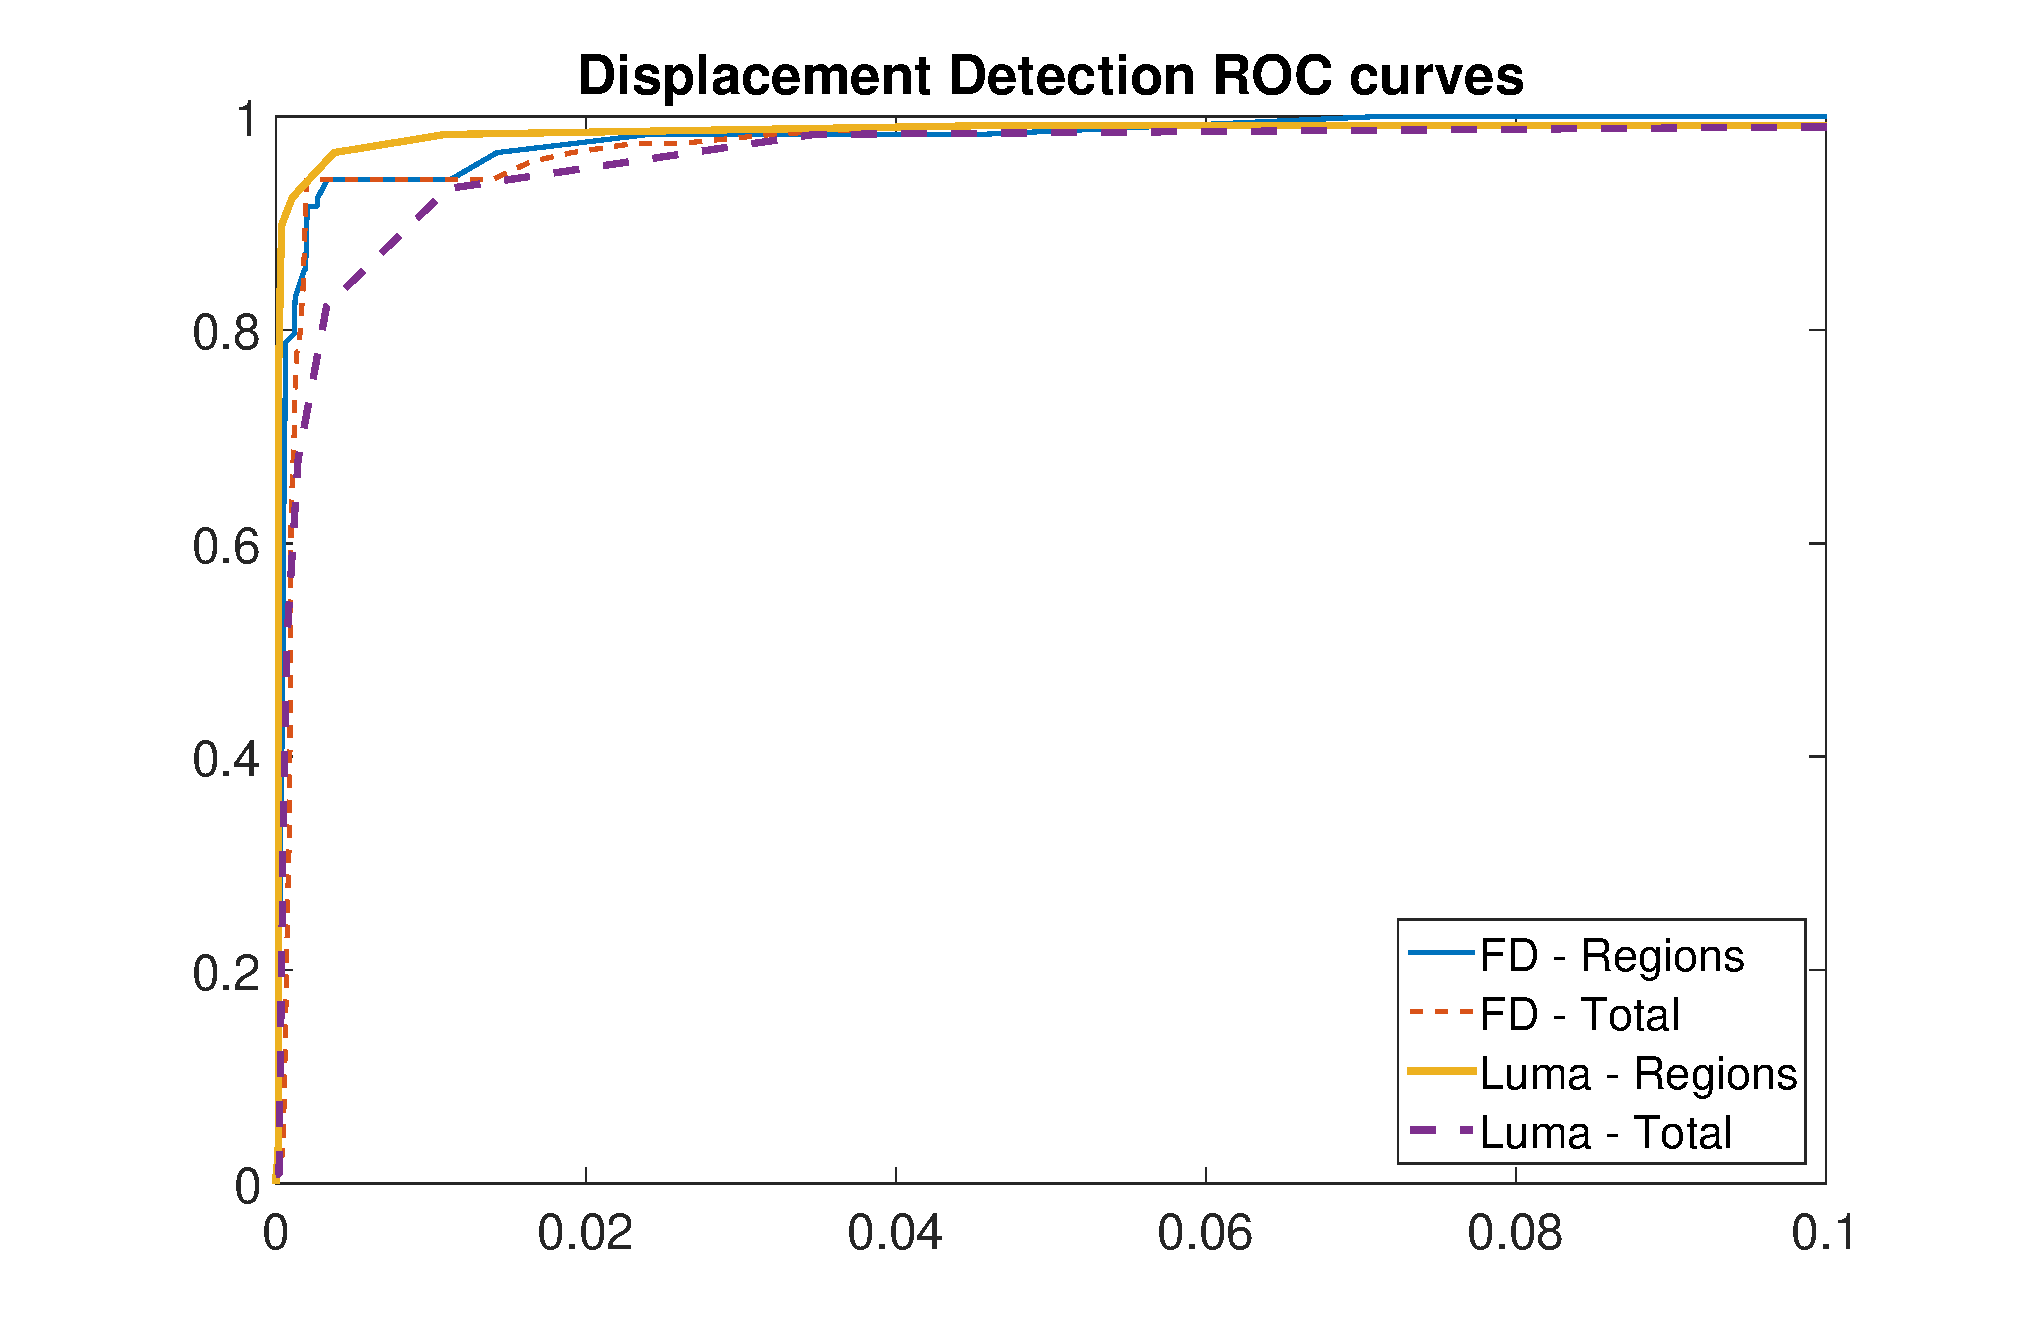
\includegraphics[width=13cm]{diagrammi/ROC_displacement}
\caption{Curve ROC per gli indicatori di spostamento della camera}
\label{fig:ROC_displacement}
\end{figure}

Per la sfocatura non abbiamo vantaggi ad utilizzare la segmentazione rispetto alla totalit\`a della scena.\\ 
\begin{figure}[tb]
\centering
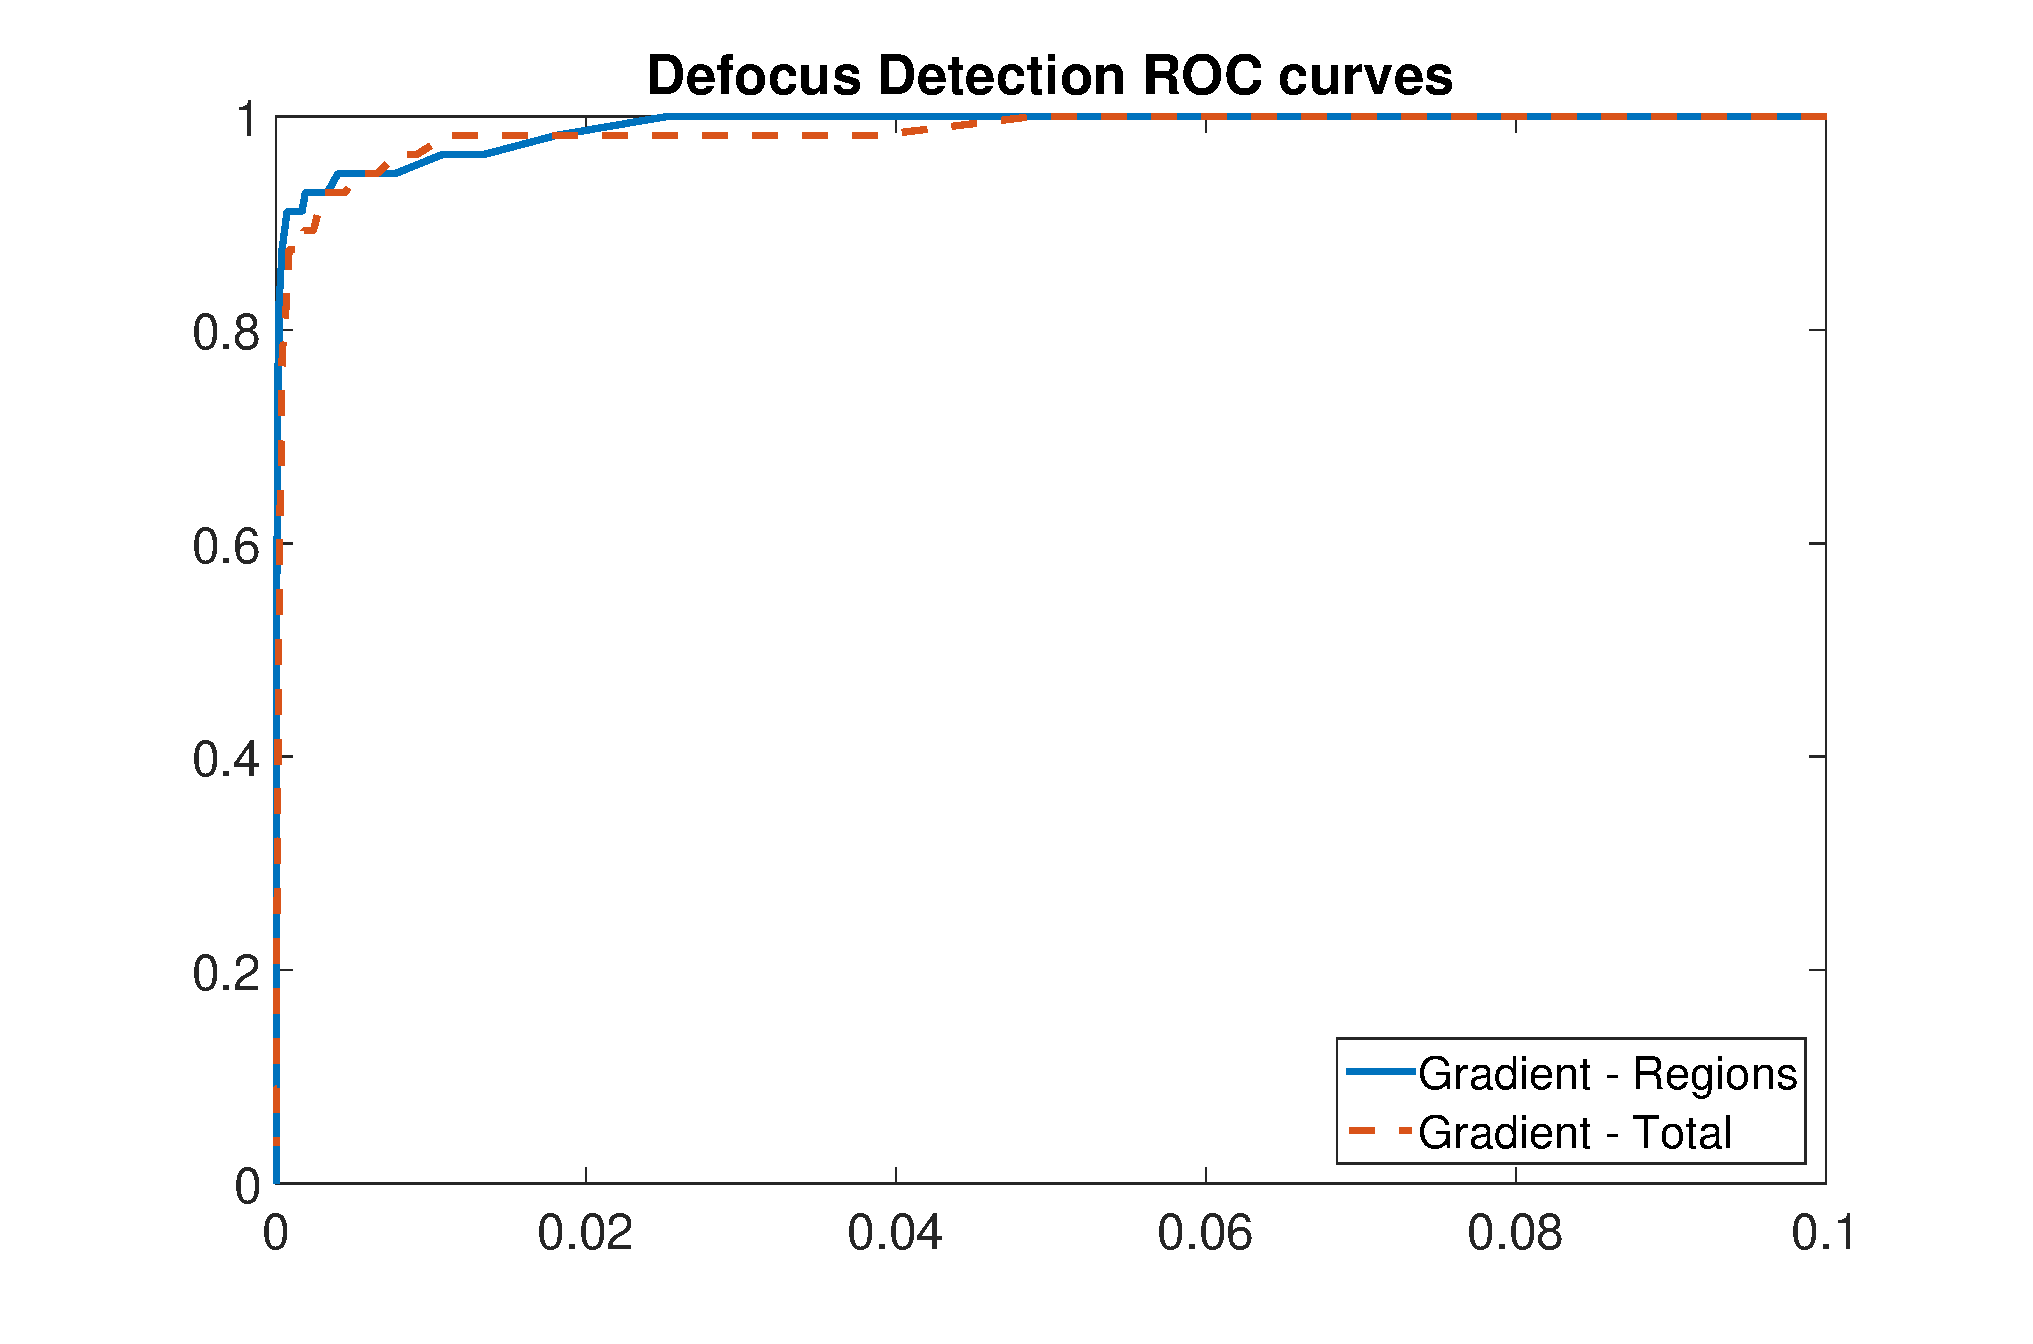
\includegraphics[width=13cm]{diagrammi/ROC_defocus}
\caption{Curve ROC per gli indicatori di sfocatura}
\label{fig:ROC_defocus}
\end{figure}

Per analizzare il monitoraggio sequenziale abbiamo visto le prestazione in base all'intensit\`a della sfocatura avvenuta (larghezza del filtro).\\
Grafici:
\begin{itemize}
	\item \textbf{Detection Delay}: differenza tra la detection dell'algoritmo e il GT
	\item \textbf{False Positive Rate} $<$- CAMBIARE NOME: Percentuale di FP rispetto al totale delle osservazioni
	\item \textbf{False Negative Rate} $<$- CAMBIARE NOME: Percentuale di FN rispetto al totale delle osservazioni
\end{itemize}
\begin{figure}[tb]
\centering
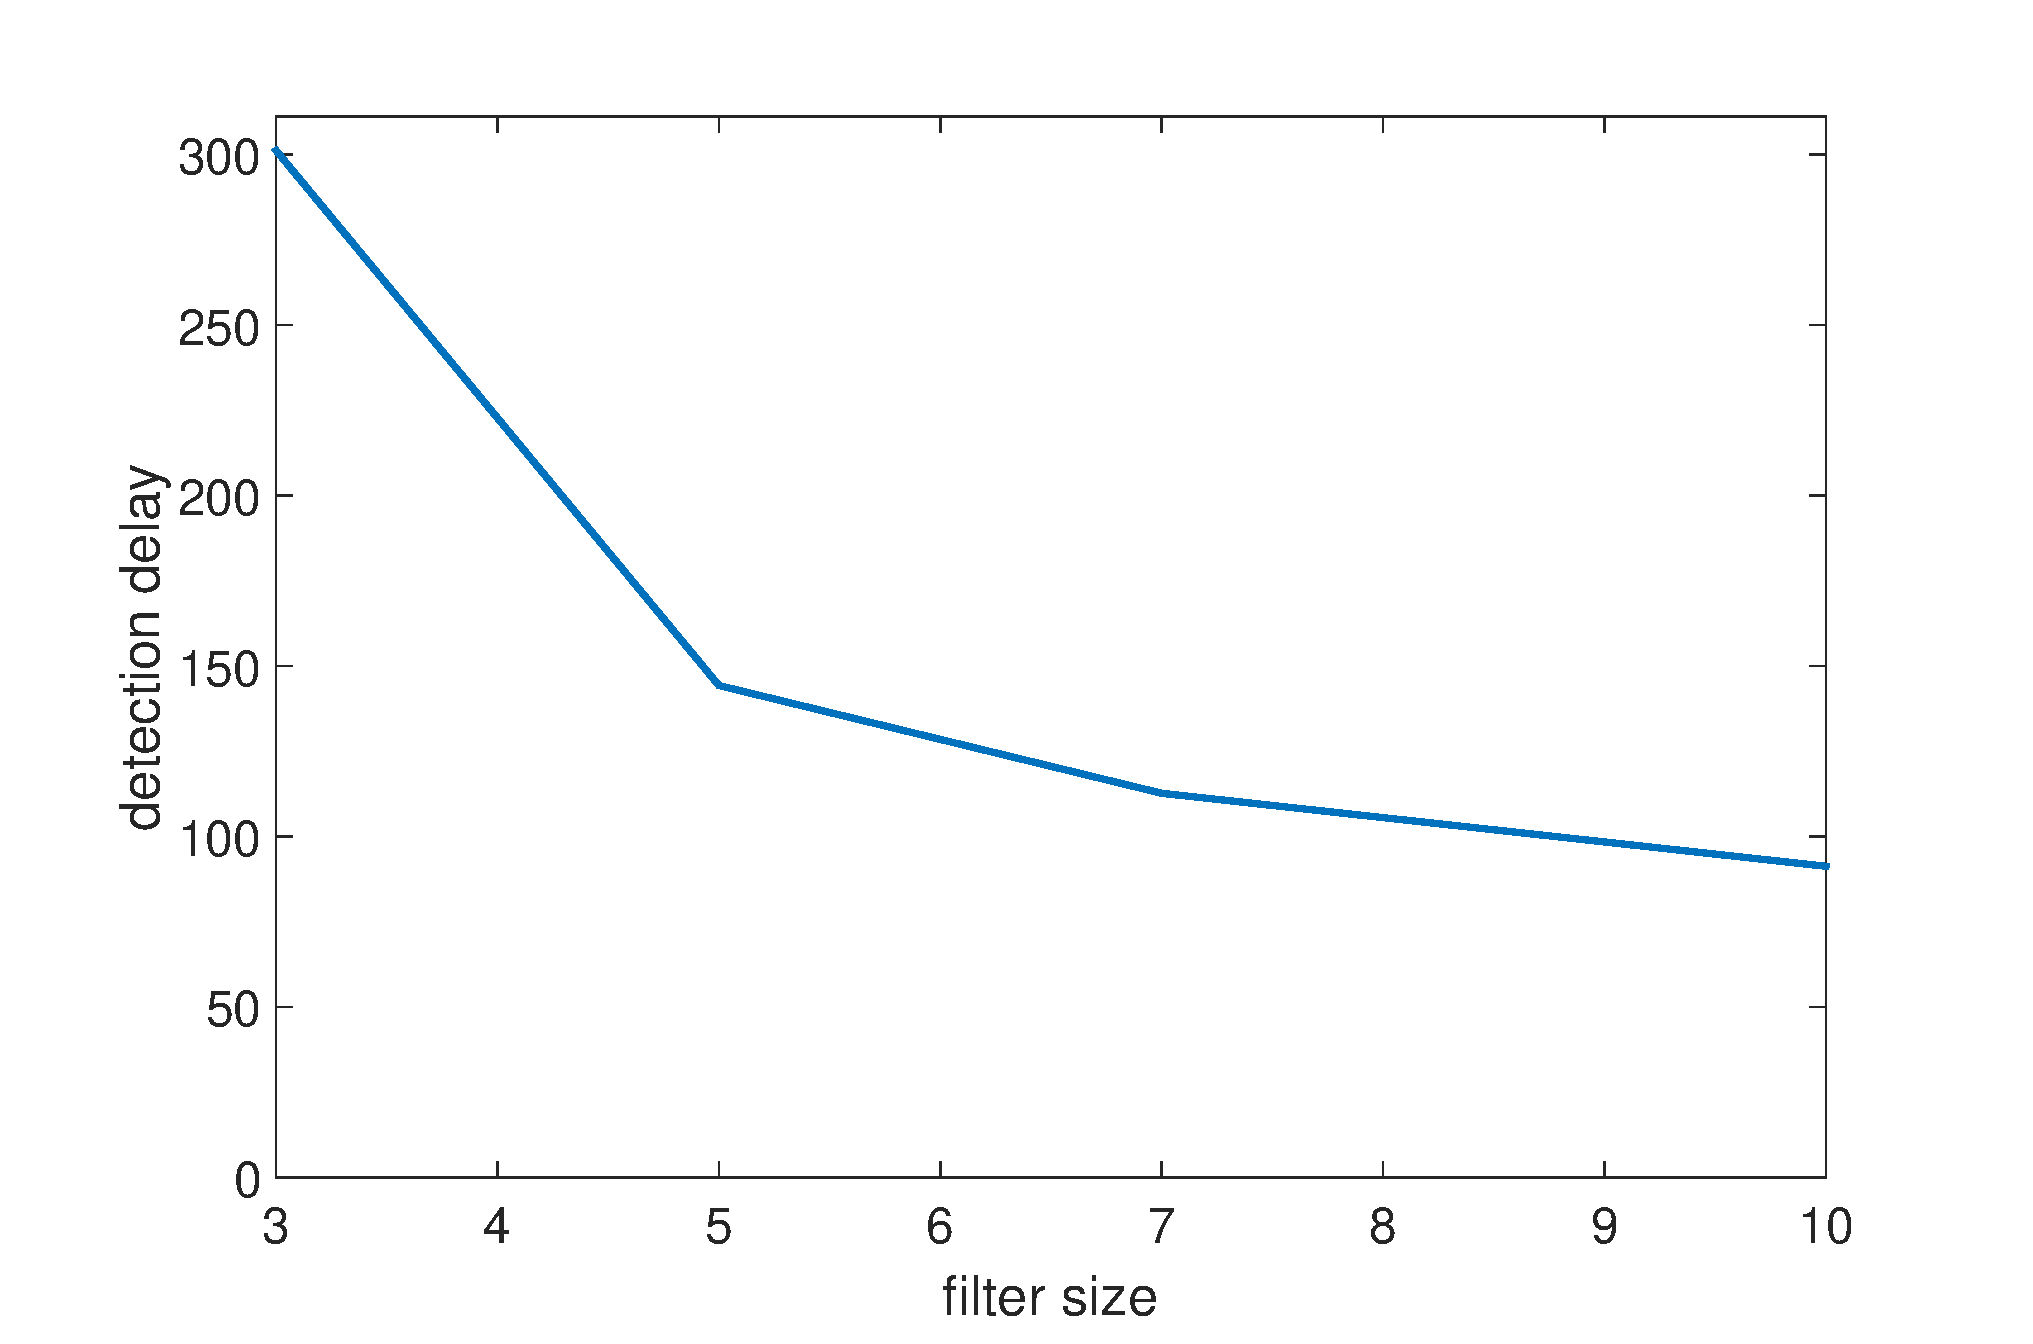
\includegraphics[width=13cm]{diagrammi/DD}
\caption{Detection Delay per l'analisi sequenziale della varianza dell'energia del gradiente}
\label{fig:DD}
\end{figure}
\begin{figure}[tb]
\centering
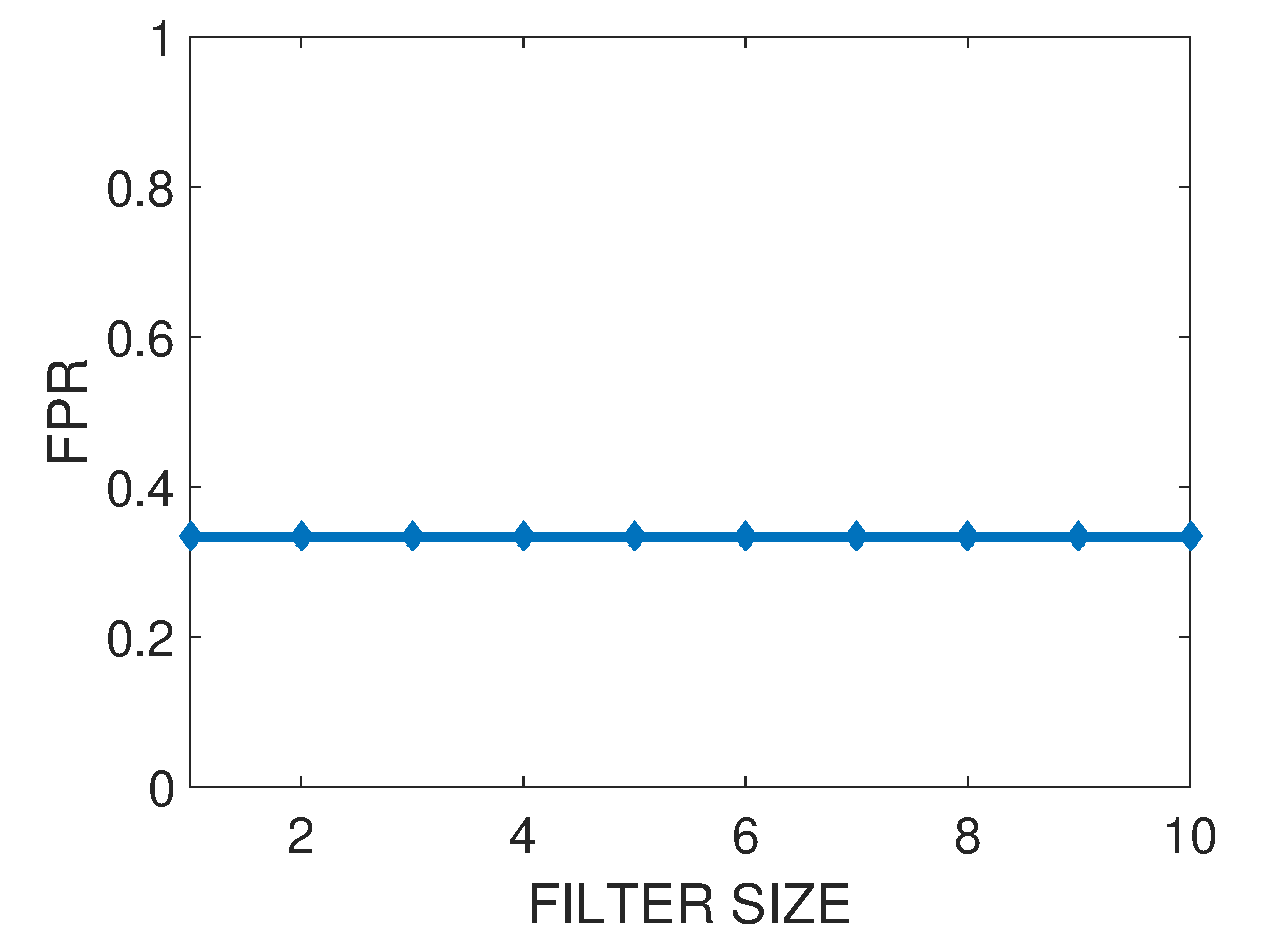
\includegraphics[width=13cm]{diagrammi/FPR}
\caption{False Positive Rate per l'analisi sequenziale della varianza dell'energia del gradiente}
\label{fig:FPR}
\end{figure}
\begin{figure}[tb]
\centering
\includegraphics[width=13cm]{diagrammi/FNR}
\caption{False Negative Rate per l'analisi sequenziale della varianza dell'energia del gradiente}
\label{fig:FNR}
\end{figure}
